\chapter{Implementation of NeuroLearn}

The NeuroLearn platform is built as a tightly integrated system combining gesture-based hardware input with an AI-driven adaptive learning backend. This chapter details the end-to-end implementation of the system across two principal layers: the physical gesture input module, which captures hand signs through a sensor-equipped glove and translates them into textual output, and the software layer, which comprises dynamic learner profiling, multi-modal content generation, and a Retrieval-Augmented Generation (RAG) pipeline. Together, these modules form a cohesive, accessibility-first educational platform that personalises content delivery based on real-time user interaction.

% ─────────────────────────────────────────────
\section{Hardware Implementation: Gesture Input Module}
% ─────────────────────────────────────────────

The gesture input module serves as the primary accessibility interface, enabling users — particularly those with motor or speech impairments — to interact with the NeuroLearn platform through hand signs. The module is designed around a fabric glove embedded with flex sensors, an Arduino microcontroller, and a character LCD display, forming a self-contained sign-to-text translation unit.

\subsection{Sensor Glove Assembly}

The base of the module is a standard fabric glove onto which five flex sensors are affixed along each finger using adhesive. Flex sensors are thin, flexible resistive elements whose electrical resistance changes proportionally when bent. When the user forms a hand sign, the corresponding fingers flex to varying degrees, causing each sensor to register a unique resistance value. This resistance variation encodes the shape and orientation of the hand gesture in a measurable electrical form.

Each flex sensor is wired in a voltage divider configuration with a \(10\,\text{k}\Omega\) fixed resistor, as illustrated in Figure~\ref{fig:voltage_divider}. The output voltage of each divider is given by:

\[
V_{\text{out}} = V_{\text{cc}} \times \frac{R_{\text{fixed}}}{R_{\text{fixed}} + R_{\text{flex}}}
\]

As the flex sensor bends and \(R_{\text{flex}}\) increases, \(V_{\text{out}}\) decreases proportionally. This analog voltage is fed into one of the Arduino's Analog-to-Digital Converter (ADC) pins, where it is sampled and quantised to a 10-bit integer in the range 0–1023.

% ── Figure 1: Voltage Divider Circuit ──────────────────
\begin{figure}[h]
	\centering
	\begin{tikzpicture}[
		circuit ee IEC,
		every resistor/.style={draw, minimum width=0.6cm, minimum height=0.25cm},
		thick, >=latex
		]
		% VCC node
		\node[above] at (0,3.5) {\(V_{\text{cc}}\,(5\,\text{V})\)};
		\draw (0,3.5) -- (0,3);
		
		% Flex sensor (top resistor) — wider + taller so label fits
		\draw (0,3) -- (0,2.5);
		\draw[fill=blue!10] (-0.9,2.5) rectangle (0.9,1.3);
		\node[font=\small] at (0,1.9) {Flex Sensor};
		\draw (0,1.3) -- (0,0.8);
		
		% Junction and output label
		\node[circle, fill=black, inner sep=1.5pt] at (0,0.8) {};
		\draw[->, dashed] (0,0.8) -- (2.4,0.8) node[right]{\(V_{\text{out}}\) \(\rightarrow\) Arduino ADC};
		
		% Fixed resistor (bottom) — wider + taller so label fits
		\draw (0,0.8) -- (0,0.2);
		\draw[fill=orange!10] (-0.9,0.2) rectangle (0.9,-0.8);
		\node[font=\small] at (0,-0.3) {\(10\,\text{k}\Omega\)};
		\draw (0,-0.8) -- (0,-1.4);
		
		% GND
		\draw (-0.35,-1.4) -- (0.35,-1.4);
		\draw (-0.22,-1.55) -- (0.22,-1.55);
		\draw (-0.09,-1.7) -- (0.09,-1.7);
		\node[below] at (0,-1.7) {GND};
	\end{tikzpicture}
	\caption{Voltage divider circuit for a single flex sensor connected to an Arduino ADC input pin.}
	\label{fig:voltage_divider}
\end{figure}

\subsection{Arduino Processing and Gesture Recognition}

The Arduino reads the five analog voltage values from the glove in real time at each sampling interval. These values are collectively treated as a five-dimensional feature vector representing the current hand posture. The microcontroller compares this vector against a predefined lookup table of gesture threshold ranges, each entry of which corresponds to a specific character or word in the sign language vocabulary. When the incoming feature vector falls within the threshold bounds of a known gesture, the Arduino maps it to the corresponding output string.

The complete hardware data flow — from sensor bending through analog sampling, gesture matching, and dual output — is illustrated in Figure~\ref{fig:hardware_flow}.

% ── Figure 2: Hardware Data Flow ───────────────────────
\begin{figure}[h]
	\centering
	\begin{tikzpicture}[
		node distance=0.55cm and 1.1cm,
		box/.style={draw, rounded corners=4pt, fill=#1, minimum width=2.5cm,
			minimum height=0.75cm, align=center, font=\small},
		arr/.style={->, thick, >=latex}
		]
		\node[box=blue!15]   (glove)  {Fabric Glove \\ + Flex Sensors};
		\node[box=orange!20, right=of glove]  (vdiv)  {Voltage \\ Divider};
		\node[box=green!15,  right=of vdiv]   (adc)   {Arduino ADC \\ (10-bit)};
		\node[box=yellow!20, right=of adc]    (match) {Gesture \\ Matching};
		\node[box=red!15,    below right=of match, yshift=0.3cm] (lcd)  {LCD Display};
		\node[box=purple!15, above right=of match, yshift=-0.3cm] (plat) {NeuroLearn \\ Platform};
		
		\draw[arr] (glove)  -- node[above,font=\tiny]{resistance} (vdiv);
		\draw[arr] (vdiv)   -- node[above,font=\tiny]{\(V_{\text{out}}\)} (adc);
		\draw[arr] (adc)    -- node[above,font=\tiny]{0–1023} (match);
		\draw[arr] (match)  -- node[right,font=\tiny]{text} (lcd);
		\draw[arr] (match)  -- node[right,font=\tiny]{text} (plat);
	\end{tikzpicture}
	\caption{End-to-end hardware data flow: from finger bending through analog sampling, gesture classification, and dual output to the LCD screen and NeuroLearn platform.}
	\label{fig:hardware_flow}
\end{figure}

\subsection{LCD Display and Feedback}

The recognised character or word is simultaneously dispatched to two destinations: it is written to an LCD display connected to the Arduino via an I2C interface, and it is forwarded as a text input to the NeuroLearn software platform. The LCD provides immediate, local visual confirmation that the gesture was captured correctly before the input travels to the adaptive learning engine. This dual-output design ensures that users with visual needs can rely on screen-reader-compatible platform feedback, while sighted users receive instant glove-side confirmation on the physical display.

% ─────────────────────────────────────────────
\section{Software Implementation}
% ─────────────────────────────────────────────

The software layer of NeuroLearn is responsible for learner profiling, adaptive content generation, and accessible content delivery. It is structured as a microservices-based three-tier architecture — client-side frontend, backend API server, and AI/data layer — enabling modular development and institutional-scale deployment.

\subsection{System Architecture}

The high-level architecture, shown in Figure~\ref{fig:system_arch}, consists of three functional tiers. The client-side frontend is built with React.js 18.2 and Material-UI, adhering strictly to WCAG 2.1 Level AAA guidelines. Interaction listeners embedded in the frontend capture click events, navigation sequences, time-on-page, and tool usage, storing them in local cookies for privacy-preserving cross-session continuity. The backend API server, implemented in Python Flask 3.0, hosts the Profile Fusion Engine and the Session Manager. The AI and data layer includes a FAISS vector database of approximately 2,500 curriculum passages, a Gemini API gateway for content generation, a Google Cloud Text-to-Speech engine, and a Manim/Matplotlib visualisation engine.

% ── Figure 3: System Architecture ──────────────────────
\begin{figure}[h]
	\centering
	\begin{tikzpicture}[
		tier/.style={draw, fill=#1, rounded corners=5pt,
			minimum width=3.2cm, minimum height=0.7cm,
			align=center, font=\small\bfseries},
		comp/.style={draw, fill=#1!10, rounded corners=3pt,
			minimum width=2.9cm, minimum height=0.6cm,
			align=center, font=\footnotesize},
		arr/.style={->, thick, >=latex, gray}
		]
		% ── Column 1: Frontend ──
		\node[tier=blue] (fe) at (0,0) {Client-Side Frontend};
		\node[comp=blue, below=0.3cm of fe] (react) {React.js UI};
		\node[comp=blue, below=0.15cm of react] (listen) {Interaction Listeners};
		\node[comp=blue, below=0.15cm of listen] (cookie) {Local Cookie Storage};
		
		% ── Column 2: Backend ──
		\node[tier=orange] (be) at (4.2,0) {Backend API Server};
		\node[comp=orange, below=0.3cm of be] (req) {Request Handler};
		\node[comp=orange, below=0.15cm of req] (pfuse) {Profile Fusion Engine};
		\node[comp=orange, below=0.15cm of pfuse] (sess) {Session Manager};
		
		% ── Column 3: AI Layer ──
		\node[tier=green] (ai) at (8.4,0) {AI \& Data Layer};
		\node[comp=green, below=0.3cm of ai] (faiss) {FAISS Vector DB};
		\node[comp=green, below=0.15cm of faiss] (gemini) {Gemini API (LLM)};
		\node[comp=green, below=0.15cm of gemini] (tts) {TTS Engine};
		\node[comp=green, below=0.15cm of tts] (viz) {Manim/Matplotlib};
		
		% Arrows between tiers
		\draw[arr] (cookie.east)  -- ++(0.45,0) |- (req.west);
		\draw[arr] (listen.east)  -- ++(0.45,0) |- (pfuse.west);
		\draw[arr] (pfuse.east)   -- ++(0.45,0) |- (faiss.west);
		\draw[arr] (sess.east)    -- ++(0.45,0) |- (gemini.west);
	\end{tikzpicture}
	\caption{High-level three-tier system architecture of NeuroLearn showing the client-side frontend, backend API server, and AI/data layer with key components.}
	\label{fig:system_arch}
\end{figure}

\subsection{Hybrid Learner Profiling Mechanism}

Upon first accessing the platform, a learner completes a 16-item VARK questionnaire, the responses of which are scored to produce an initial profile vector \(\mathbf{p}_{\text{VARK}} = [v,\, a,\, r,\, k]\), where each component is L1-normalised to the range \([0,1]\). As the learner interacts with content over successive sessions, the backend accumulates a behavioural profile vector \(\mathbf{p}_{\text{behavior}}\) derived from interaction frequency and dwell time per modality. A weighted dynamic fusion scheme merges both signals:

\[
\mathbf{p}_{\text{final}} = \alpha(n)\,\mathbf{p}_{\text{VARK}} + \bigl(1-\alpha(n)\bigr)\,\mathbf{p}_{\text{behavior}},
\quad \alpha(n) = e^{-0.15\,n}
\]

where \(n\) is the session count. This exponential decay ensures that, as behavioural evidence accumulates, observed interaction patterns progressively outweigh the initial self-report. The dominant modality \(M_{\text{dominant}} = \arg\max_m\, p^{(m)}_{\text{final}}\) then drives all downstream content generation. The profiling convergence trajectory is depicted in Figure~\ref{fig:profiling_accuracy}.

% ── Figure 4: Profiling Accuracy ───────────────────────
\begin{figure}[htbp]
	\centering
	\begin{tikzpicture}
		\begin{axis}[
			width=9cm, height=5.5cm,
			xlabel={Session Number},
			ylabel={Profiling Accuracy (\%)},
			xmin=0.5, xmax=10.5,
			ymin=60, ymax=100,
			xtick={1,3,5,7,10},
			ytick={60,70,80,90,100},
			grid=major,
			grid style={dashed, gray!40},
			legend pos=south east,
			legend style={font=\small},
			tick label style={font=\small},
			label style={font=\small},
			]
			
			% Hybrid profiling curve
			\addplot[color=blue!70!black, mark=square*, thick]
			coordinates {(1,68.4)(3,78.2)(5,86.7)(7,90.3)(10,92.1)};
			\addlegendentry{Hybrid Profiling}
			
			% VARK-only baseline
			\addplot[color=red!70!black, mark=*, dashed, thick]
			coordinates {(1,68.4)(3,68.4)(5,68.4)(7,68.4)(10,68.4)};
			\addlegendentry{VARK-Only Baseline}
			
			% 1. Define Upper Boundary First
			\addplot[name path=upper, draw=none]
			coordinates {(1,76.6)(3,85.1)(5,92.6)(7,95.4)(10,96.6)};
			
			% 2. Define Lower Boundary Second
			\addplot[name path=lower, draw=none]
			coordinates {(1,60.2)(3,71.3)(5,80.8)(7,85.2)(10,87.6)};
			
			% 3. Fill Between AFTER defining them
			\addplot[blue!15, fill opacity=0.35] fill between[of=upper and lower];
		\end{axis}
	\end{tikzpicture}
	\caption{Profiling accuracy convergence across 10 learning sessions comparing the NeuroLearn hybrid dynamic profiling approach against the static VARK-only baseline. The shaded region represents the 95\% confidence interval.}
	\label{fig:profiling_accuracy}
\end{figure}

\subsection{Multi-Modal Content Generation Engine}

Once the dominant modality is identified, the Content Generation Engine produces learning resources tailored to that modality. For \textbf{Reading/Writing} learners, structured summaries are generated using BART-large-CNN and comprehensive text explanations via the Gemini API, supplemented by spaced-repetition flashcards. \textbf{Auditory} learners receive neural text-to-speech audio explanations generated through Google Cloud TTS with WaveNet voices, alongside voice-controlled dialogue interfaces. \textbf{Visual} learners are presented with concept maps rendered by Matplotlib, graphical mind maps from Graphviz, and animated step-by-step explanations produced through Manim Community Edition. \textbf{Kinesthetic} learners access interactive coding sandboxes, drag-and-drop exercises, and topic simulations. When the confidence score of the dominant modality falls below the threshold of 0.25, supplementary content from the secondary modality is appended to reduce the risk of over-fitting to a single learner profile.

\subsection{Modality-Aware Retrieval-Augmented Generation Pipeline}

To ensure curricular accuracy and minimise hallucination, NeuroLearn employs a Retrieval-Augmented Generation (RAG) pipeline, illustrated in Figure~\ref{fig:rag_pipeline}. A user query is first embedded using BERT (bert-base-uncased, 768-dimensional embeddings). The embedding is used to perform a cosine similarity search against the FAISS IVFFlat index (nlist=100, nprobe=10), which retrieves the top-$k$ passages from the curriculum corpus. Passages with a similarity score below 0.6 are rejected as out-of-scope. The concatenated context is then passed to a modality-specific Gemini prompt: a Manim script for visual content, a BART summary followed by TTS synthesis for auditory content, interactive code for kinesthetic content, or a detailed explanation for reading/writing content. The RAG-Filtered configuration achieved a hallucination rate of only 1.3\% compared to 12.7\% for pure LLM generation, with an average query latency of 24.3\,ms at the FAISS layer and an overall response time of 1.8\,s.

% ── Figure 5: RAG Pipeline ─────────────────────────────
\begin{figure}[h]
	\centering
	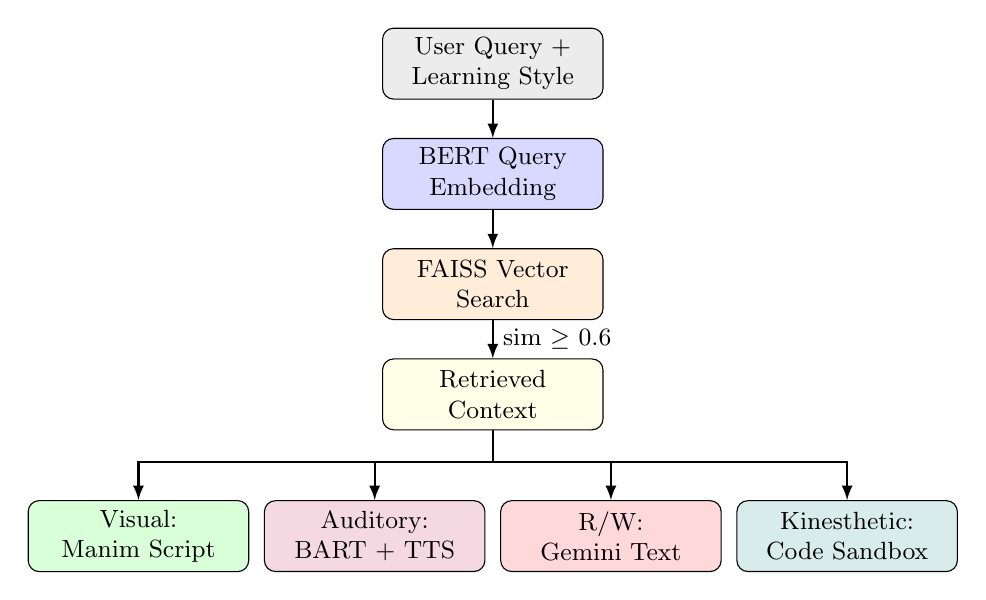
\begin{tikzpicture}[
		box/.style={draw, rounded corners=4pt, fill=#1,
			minimum width=2.8cm, minimum height=0.9cm,
			align=center, font=\small},
		arr/.style={->, thick, >=latex}
		]
		% Shared spine — centred at x=0
		\node[box=gray!15]   (query)  at (0, 0)    {User Query +\\ Learning Style};
		\node[box=blue!15]   (embed)  at (0,-1.4)  {BERT Query\\ Embedding};
		\node[box=orange!15] (search) at (0,-2.8)  {FAISS Vector\\ Search};
		\node[box=yellow!10] (ctx)    at (0,-4.2)  {Retrieved\\ Context};
		
		% Four modality branches — evenly spread with enough gap
		\node[box=green!15]  (vis) at (-4.5,-6.0) {Visual:\\ Manim Script};
		\node[box=purple!15] (aud) at (-1.5,-6.0) {Auditory:\\ BART + TTS};
		\node[box=red!15]    (rw)  at ( 1.5,-6.0) {R/W:\\ Gemini Text};
		\node[box=teal!15]   (kin) at ( 4.5,-6.0) {Kinesthetic:\\ Code Sandbox};
		
		% Arrows
		\draw[arr] (query)  -- (embed);
		\draw[arr] (embed)  -- (search);
		\draw[arr] (search) -- node[right,font=\small]{sim $\geq$ 0.6} (ctx);
		\draw[arr] (ctx.south) -- ++(0,-0.4) -| (vis.north);
		\draw[arr] (ctx.south) -- ++(0,-0.4) -| (aud.north);
		\draw[arr] (ctx.south) -- ++(0,-0.4) -| (rw.north);
		\draw[arr] (ctx.south) -- ++(0,-0.4) -| (kin.north);
	\end{tikzpicture}
	\caption{Modality-aware Retrieval-Augmented Generation (RAG) pipeline in NeuroLearn. Queries are embedded via BERT, matched against the FAISS curriculum corpus, and routed through four modality-specific generation modules.}
	\label{fig:rag_pipeline}
\end{figure}

\subsection{Accessibility-First Adaptation}

Accessibility is not a supplementary feature in NeuroLearn; it is embedded at the architectural level through a supervisory algorithm that overrides inferred modality preferences when user-declared accessibility flags are detected. Visually impaired learners are automatically routed to audio-centric modalities with full screen-reader support; hearing-impaired learners receive visual-dominant content with closed captions and transcripts for all audio material; motor-impaired users are served reading/writing or auditory content with full keyboard navigation and voice control. Color contrast across the interface conforms to WCAG-AAA standards, and every interactive feature supports keyboard-only access. This accessibility-first routing produced a learning gain of +24.6\% for users with declared accessibility needs, compared to +9.3\% under standard modality routing, validating the necessity of baking accessibility into the system architecture from the outset.

\subsection{Deployment and Scalability}

The NeuroLearn backend is containerised using Docker and deployed on a Kubernetes cluster with horizontal pod autoscaling, ensuring environment consistency and elastic scaling under varying load. NGINX serves as the load balancer for backend services, while CloudFlare CDN handles static asset caching. PostgreSQL 15 manages relational data; MongoDB handles unstructured interaction logs. The system sustained 97.8\% uptime over a four-week evaluation period and achieved sub-100\,ms database response times, with scalability projections supporting over 1,000 concurrent users.

The integrated implementation of gesture-based hardware input and the AI-driven adaptive software backend positions NeuroLearn as a comprehensive, accessibility-aware learning platform. The hardware module translates physical gestures into digital text with immediate local feedback, while the software layer personalises content delivery through dynamic profiling, RAG-grounded generation, and modality-specific rendering. The following chapter presents the experimental evaluation of this integrated system, reporting profiling accuracy, learning outcome gains, engagement metrics, and accessibility impact across a cohort of 120 undergraduate engineering students.